\section{Real-Time Validation and Results}
The process used for real-time validation is the same as chapter \ref{A8_cahp}. The CHIL testbed and controller hardware setup was the same. The model used in the DRTS was modeled using the same methodologies. The real-time validation also uses the same DNP3 communication over TCP/IP. For the first CHIL validation, the one day simulation scenario using the NYISO RTP described in the previous section was used. Fig. \ref{fig:OFFLINE1_NM_ES1_Z_RT} shows the real-time vs offline responses comparison for ES1. The blue solid line is the offline response and the dotted black line is the real-time response. The responses differ 0.3\% which is negligible. Fig. \ref{fig:OFFLINE1_NM_ES2_Z_RT}, and fig. \ref{fig:OFFLINE1_NM_GEN_Z_RT} shows the offline vs real-time responses for ES2 and the generator. In both cases, the dotted black line is the real-time response and the solid blue line is the offline response. They show a difference of 0.13\% and 0.014\% respectively. This is expected as similar to Chapter \ref{A8_cahp} offline simulation models were modeled for phasor simulation and the real-time simulation models were modeled for electromagnetic transient program simulation.

\begin{figure}[!ht]
\centering
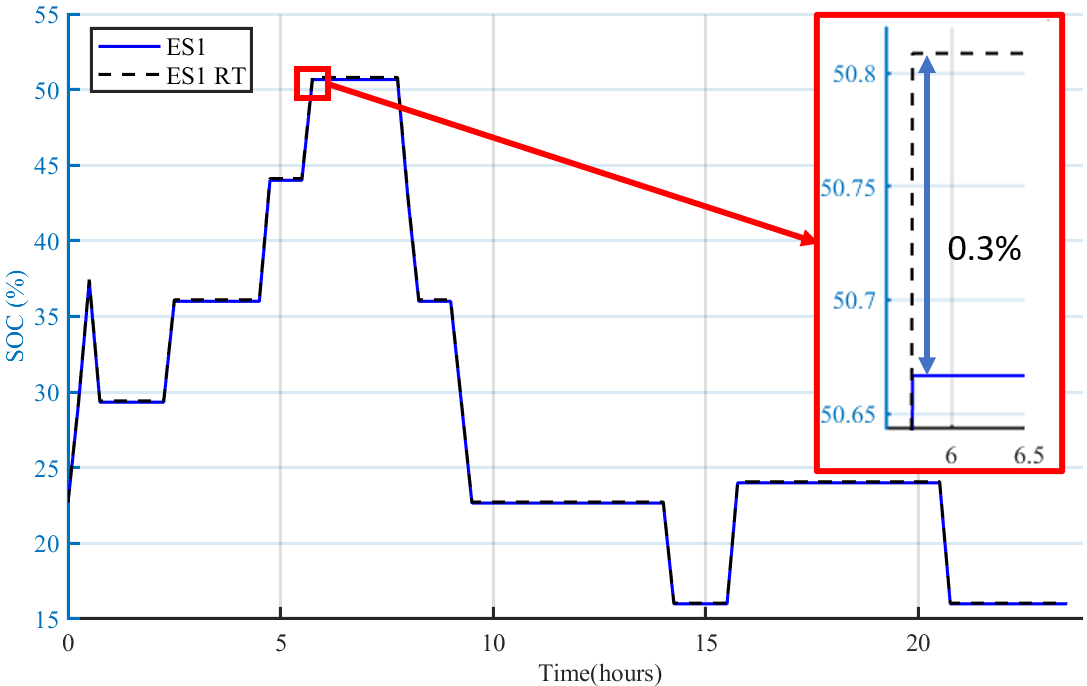
\includegraphics[width = \linewidth]{figs/A82/OFFLINE1_NM_ES1_Z_RT.png}
\caption{Comparison between ES1 responses, real-time vs offline (NYISO).}
\label{fig:OFFLINE1_NM_ES1_Z_RT}
\end{figure}

\begin{figure}[!ht]
\centering
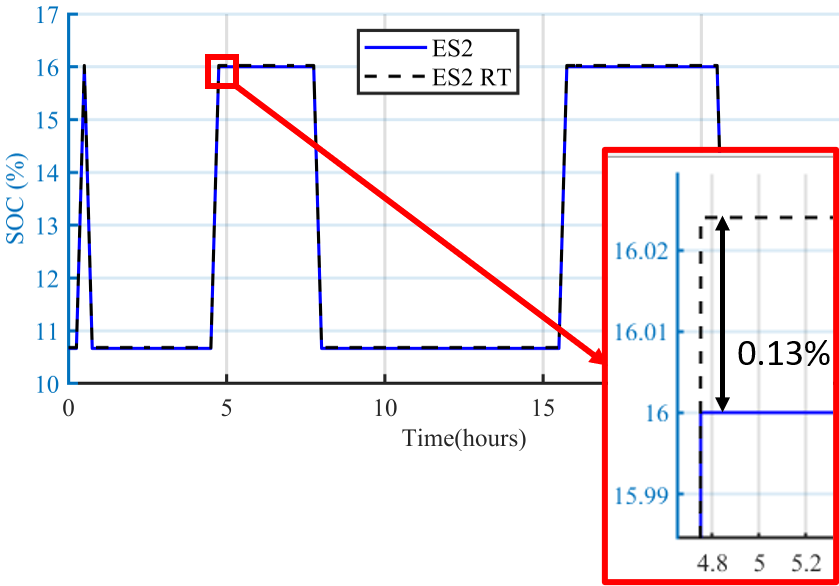
\includegraphics[width = \linewidth]{figs/A82/OFFLINE1_NM_ES2_Z_RT.png}
\caption{Comparison between ES2 responses, real-time vs offline (NYISO).}
\label{fig:OFFLINE1_NM_ES2_Z_RT}
\end{figure}

\begin{figure}[!ht]
\centering
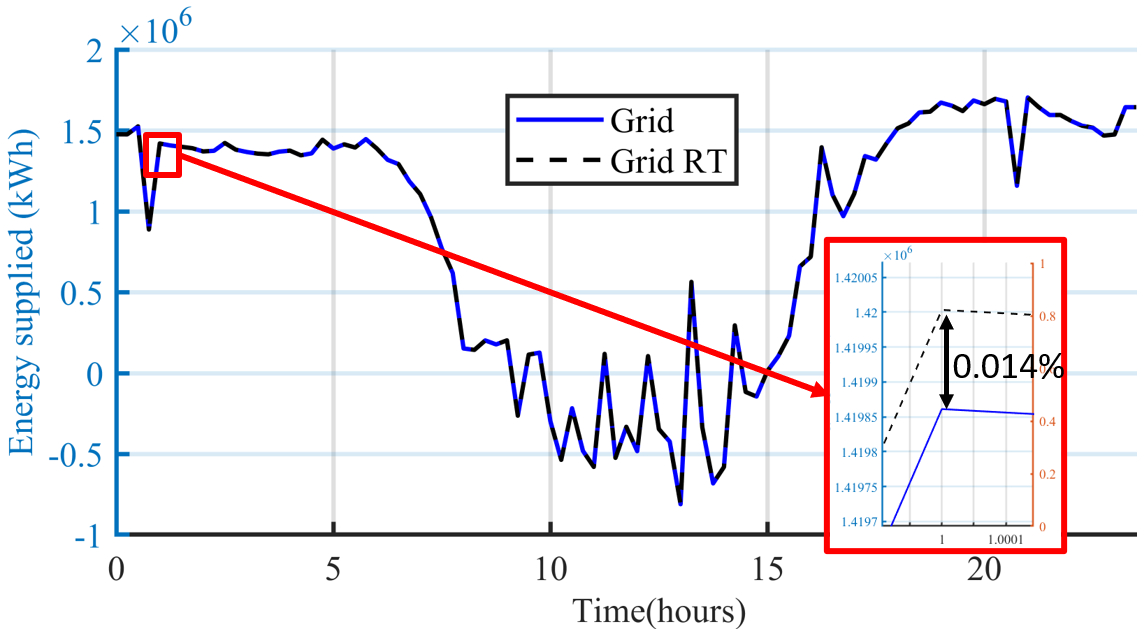
\includegraphics[width = \linewidth]{figs/A82/OFFLINE1_NM_GEN_Z_RT.png}
\caption{Comparison between generator responses, real-time vs offline (NYISO).}
\label{fig:OFFLINE1_NM_GEN_Z_RT}
\end{figure}

The second CHIL validation uses the PG\&E based RTP. Fig. \ref{fig:PGNE1_NM_ES1_Z_RT}, Fig. \ref{fig:PGNE1_NM_ES2_Z_RT}, and Fig. \ref{fig:PGNE1_NM_GEN_Z_RT} shows the offline and real-time response for ES1, ES2, and the generator, respectively. The dotted black line represents the real-time response and the solid blue line represents the off-line response in all the figures. The offline vs real-time difference for ES1, ES2, and generator are 0.2\%, 0.25\%, and 0.017\% respectively. These differences are negligible. This verifies the algorithm's capabilities to operate in a real-time environment.

\begin{figure}[!ht]
\centering
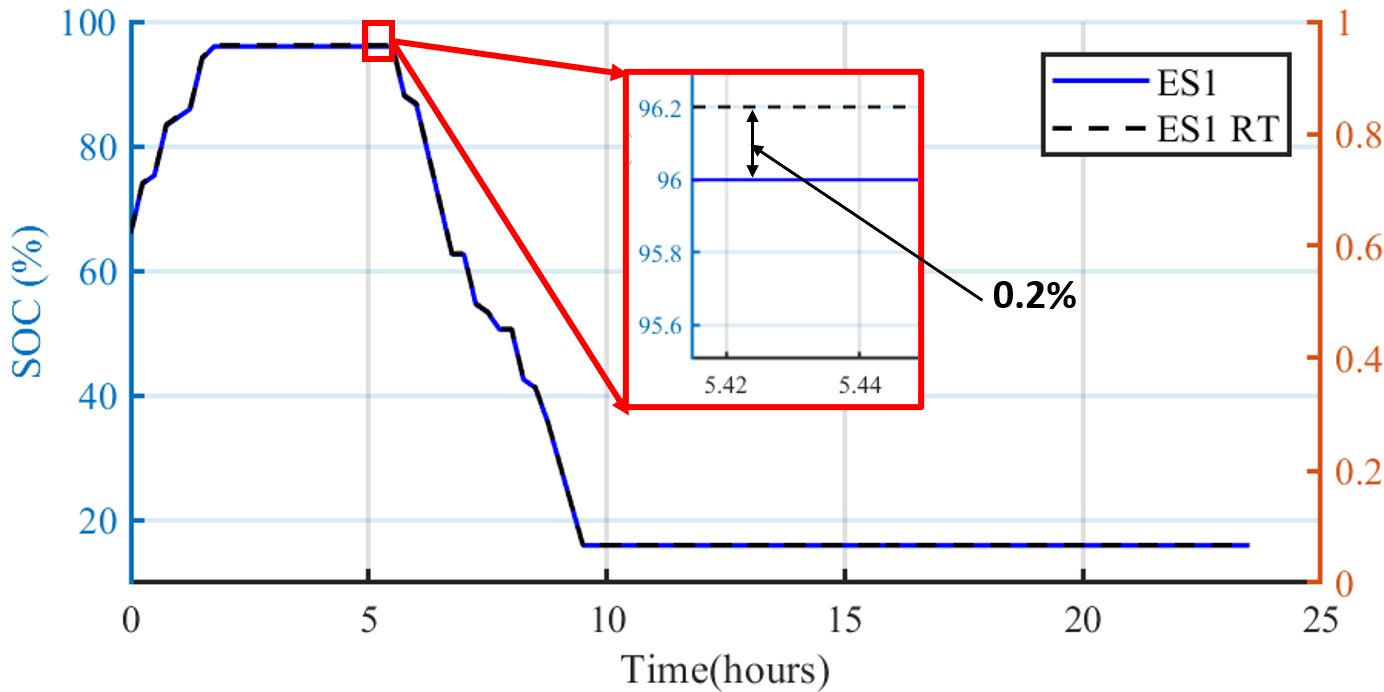
\includegraphics[width = \linewidth]{figs/A82/PGNE_RT_OFF_ES1.png}
\caption{Comparison between ES1 responses, real-time vs offline (PG\&E).}
\label{fig:PGNE1_NM_ES1_Z_RT}
\end{figure}

\begin{figure}[!ht]
\centering
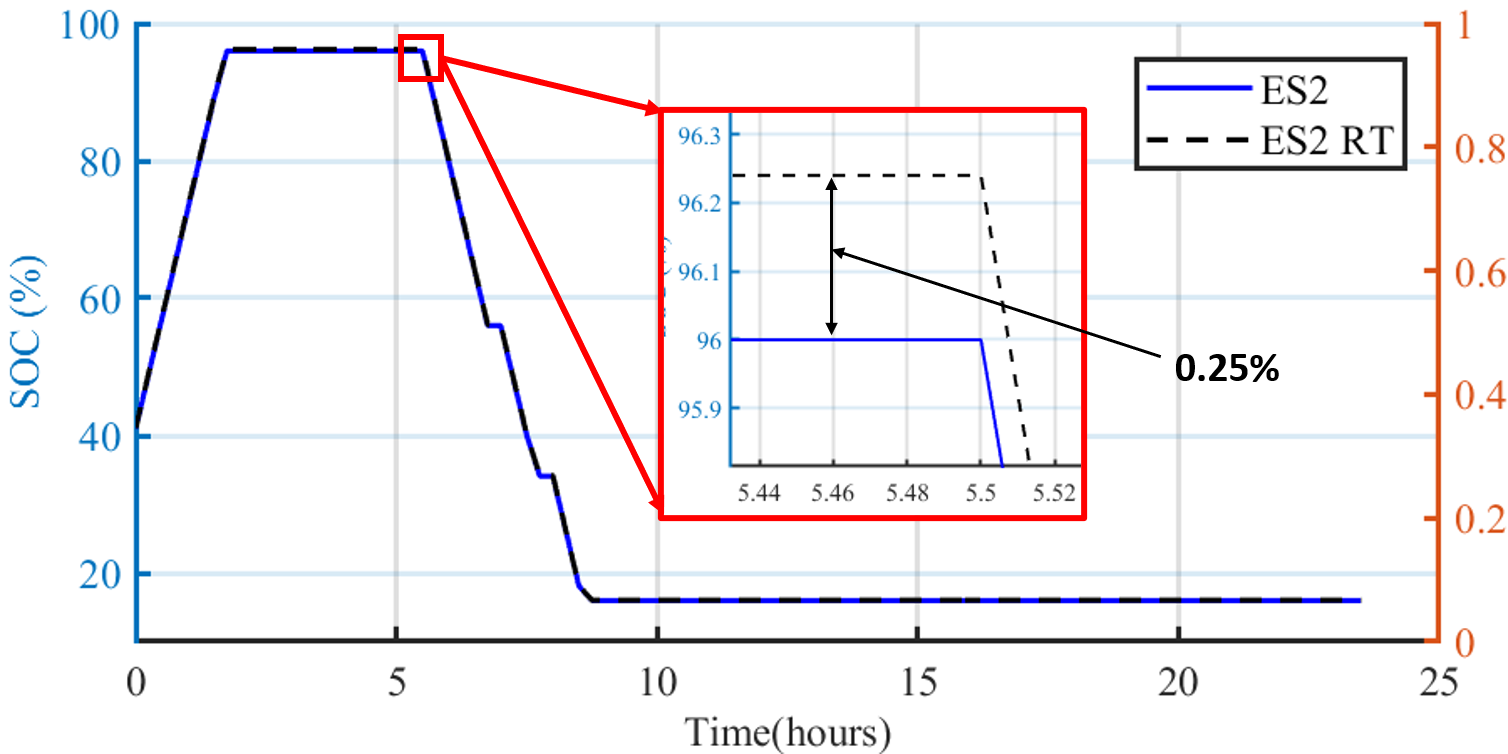
\includegraphics[width = \linewidth]{figs/A82/PGNE_RT_OFF_ES2.png}
\caption{Comparison between ES2 responses, real-time vs offline (PG\&E).}
\label{fig:PGNE1_NM_ES2_Z_RT}
\end{figure}

\begin{figure}[!ht]
\centering
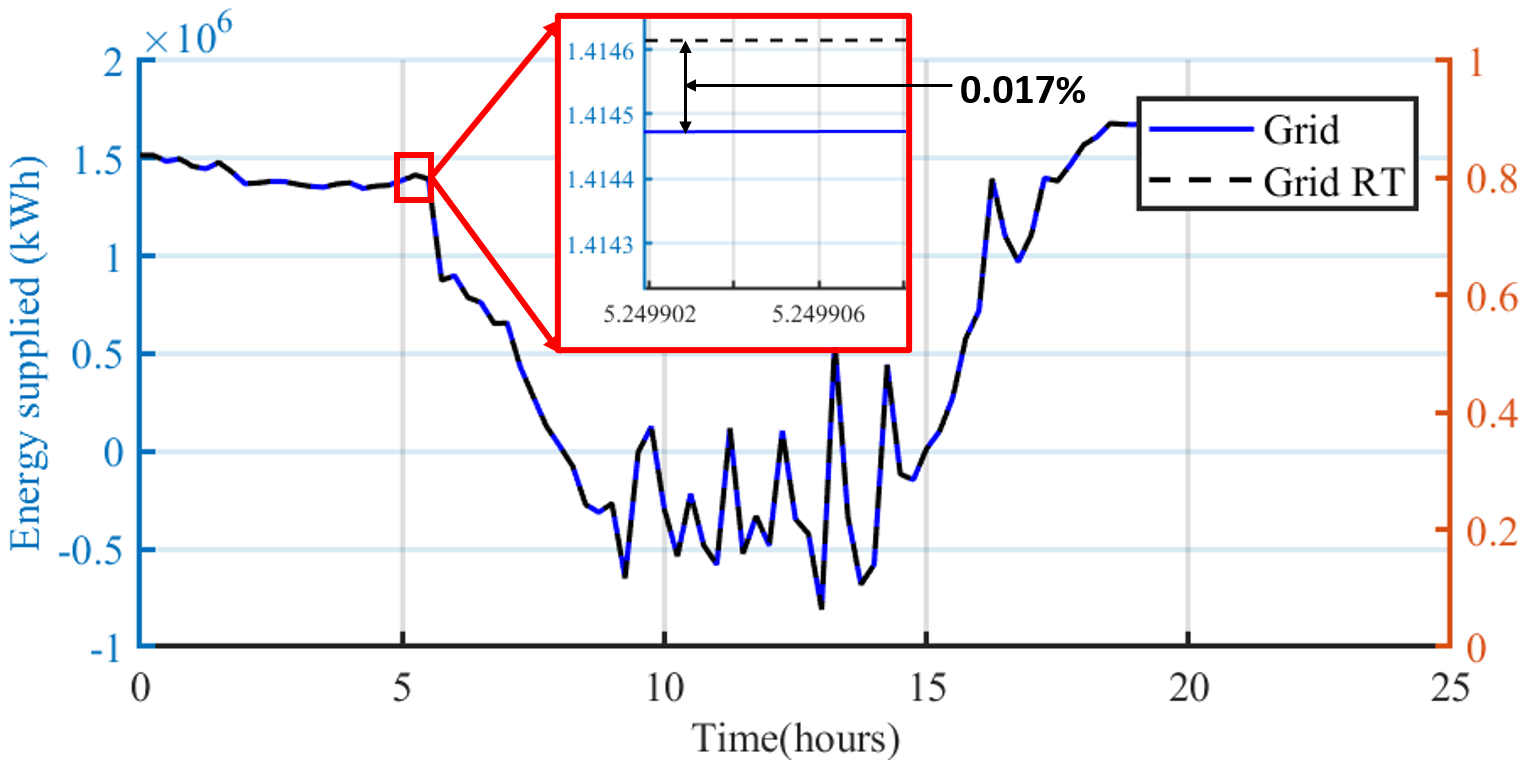
\includegraphics[width = \linewidth]{figs/A82/PGNE_RT_OFF_GEN.png}
\caption{Comparison between generator responses, real-time vs offline (PG\&E).}
\label{fig:PGNE1_NM_GEN_Z_RT}
\end{figure}